\documentclass[pdflatex,sn-mathphys-num]{sn-jnl}

\usepackage{bookmark}
\usepackage{tabularx}
\usepackage{tikz}
\usetikzlibrary{shapes.geometric, shapes.misc, arrows.meta, positioning, calc}
\usepackage{graphicx}
\usepackage{multirow}
\usepackage{amsmath,amssymb,amsfonts}
\usepackage{booktabs}

\raggedbottom

\renewcommand{\thefigure}{S\arabic{figure}}
\renewcommand{\thetable}{S\arabic{table}}

\begin{document}

\title[Supplementary material: CNN piano chord recognition]{Supplementary material: Evaluating a CNN for Piano Chord Recognition Under Factorized Acoustic Domain Shift}

\author*[1]{\fnm{Cikal} \sur{Gemintang Seya}}\email{cikalgemintangseya1@gmail.com}
\author[1]{\fnm{Jasman} \sur{Pardede}}\email{jasman@itenas.ac.id}
\affil*[1]{\orgdiv{Informatics}, \orgname{National Institute of Technology}, \orgaddress{\street{Neglasari}, \city{Bandung}, \postcode{40124}, \state{West Java}, \country{Indonesia}}}

\maketitle

This supplement documents the MIDI recorder, the six recorded datasets, CNN training, and extra domain-shift views that do not fit in the main article. Dataset identifiers match the main text: \texttt{training}, \texttt{thinkpad}, \texttt{vivo}, \texttt{flow}, \texttt{thinkpad-2}, \texttt{flow-2}.

\section{Dataset generator}

All six datasets were captured with the same web recorder. The browser talks to the keyboard over USB MIDI and to one microphone at a time. Fig.~\ref{fig:esm-app} is the session screen. Fig.~\ref{fig:esm-flow} is the capture loop.

\begin{figure}[t]
\centering
\includegraphics[width=0.92\textwidth]{ESM_1.png}
\caption{Web recorder used for every dataset. USB MIDI drives the keyboard; the selected microphone writes a labeled clip.}
\label{fig:esm-app}
\end{figure}

\begin{figure}[t]
  \centering
  \resizebox{!}{0.70\textheight}{%
  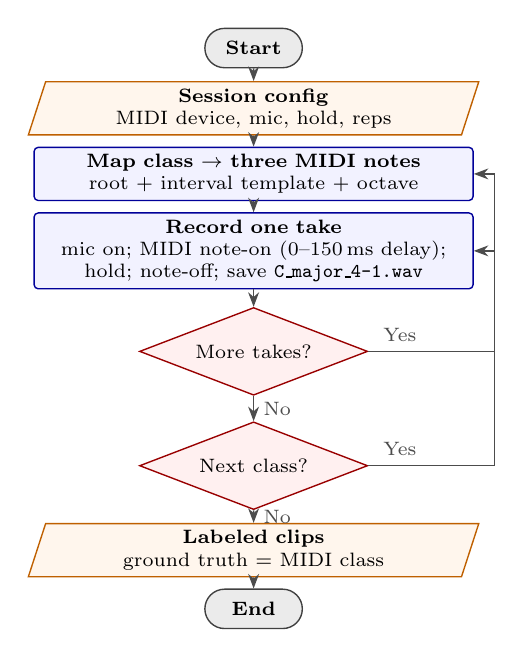
\begin{tikzpicture}[
    node distance=0.11cm and 0.10cm,
    >={Stealth},
    font=\scriptsize,
    base/.style={draw, align=center, minimum height=0.42cm, line width=0.5pt, inner sep=2.5pt},
    terminal/.style={base, shape=rounded rectangle, rounded rectangle arc length=180, draw=black!75, fill=black!8, minimum height=0.50cm, minimum width=1.8cm, inner xsep=8pt, font=\scriptsize\bfseries},
    process/.style={base, rectangle, rounded corners=1.5pt, draw=blue!60!black, fill=blue!5, text width=5.4cm},
    io/.style={base, trapezium, trapezium left angle=72, trapezium right angle=108, trapezium stretches body=true, draw=orange!75!black, fill=orange!7, text width=5.0cm, inner xsep=4pt},
    decision/.style={base, diamond, aspect=2.6, draw=red!60!black, fill=red!6, text width=2.2cm, inner sep=1pt},
    arrow/.style={->, line width=0.5pt, black!70}
  ]
    \node[terminal] (start) {Start};
    \node[io, below=0.16cm of start] (cfg)
    {\textbf{Session config}\\
     MIDI device, mic, hold, reps};
    \node[process, below=0.14cm of cfg] (map)
    {\textbf{Map class $\to$ three MIDI notes}\\
     root $+$ interval template $+$ octave};
    \node[process, below=0.14cm of map] (rec)
    {\textbf{Record one take}\\
     mic on; MIDI note-on (0--150\,ms delay);\\
     hold; note-off; save \texttt{C\_major\_4-1.wav}};
    \node[decision, below=0.22cm of rec] (morep)
    {More takes?};
    \node[decision, below=0.32cm of morep] (morec)
    {Next class?};
    \node[io, below=0.16cm of morec] (doneio)
    {\textbf{Labeled clips}\\
     ground truth $=$ MIDI class};
    \node[terminal, below=0.14cm of doneio] (endn) {End};
    \draw[arrow] (start) -- (cfg);
    \draw[arrow] (cfg) -- (map);
    \draw[arrow] (map) -- (rec);
    \draw[arrow] (rec) -- (morep);
    \draw[arrow] (morep.east) -- ++(1.6,0) node[above, font=\scriptsize, pos=0.25] {Yes}
      |- (rec.east);
    \draw[arrow] (morep) -- (morec) node[midway, right, font=\scriptsize] {No};
    \draw[arrow] (morec.east) -- ++(1.6,0) node[above, font=\scriptsize, pos=0.25] {Yes}
      |- (map.east);
    \draw[arrow] (morec) -- (doneio) node[midway, right, font=\scriptsize] {No};
    \draw[arrow] (doneio) -- (endn);
  \end{tikzpicture}%
  }
  \caption{Recorder loop. Class identity comes from the MIDI trigger, not from a human label after the fact.}
  \label{fig:esm-flow}
\end{figure}

Table~\ref{tab:esm-session} lists the session settings shared by every dataset.

\begin{table}[t]
\caption{Recorder session settings.}\label{tab:esm-session}
\begin{tabular}{@{}ll@{}}
\toprule
Parameter & Value \\
\midrule
Trigger & USB MIDI note-on (three notes) \\
Vocabulary & 12 roots $\times$ maj / min / dim, fourth octave \\
Voice & Grand-piano preset \\
Attack delay & 0--150\,ms (training) \\
Sample rate & 48{,}000\,Hz, mono \\
Training format & OGG/OPUS, 32-bit \\
Eval format & WAV \\
CQT window & first 2.0\,s of each clip \\
\bottomrule
\end{tabular}
\end{table}

\section{Dataset characteristics}

Table~\ref{tab:esm-inventory} is the inventory. Every dataset has all 36 classes and a constant take count (200 or 40). No class folder is missing. Durations sit above the 2.0\,s CQT crop. ThinkPad recordings are quieter than Vivo and Flow. Training CQT centroids sit higher ($\approx$467\,Hz) than the held-out sets ($\approx$269--323\,Hz).

Sixteen training clips are digital silence (peak $=0$). They remain in the 7{,}200-take set; resubstitution is still 0.9999. Vivo has 489 near-clip takes (hotter phone mic). No dataset has hard clipping (\texttt{flag\_clip} $=0$).

\begin{table}[t]
\caption{Recorded datasets. Per-class count is constant. Duration and RMS are over all takes.}\label{tab:esm-inventory}
\setlength{\tabcolsep}{3.2pt}
\begin{tabular}{@{}llrrrrrr@{}}
\toprule
Dataset & Fmt & $N$ & /cls & Dur.\ min & Dur.\ mean & RMS dB & Cent.\ Hz \\
\midrule
\texttt{training} & OGG & 7{,}200 & 200 & 2.00 & 2.40 & $-21.4$ & 467 \\
\texttt{thinkpad} & WAV & 1{,}440 & 40 & 2.10 & 2.45 & $-26.6$ & 323 \\
\texttt{vivo} & WAV & 1{,}440 & 40 & 2.10 & 2.44 & $-19.2$ & 290 \\
\texttt{flow} & WAV & 1{,}440 & 40 & 2.10 & 2.44 & $-19.6$ & 269 \\
\texttt{thinkpad-2} & WAV & 1{,}440 & 40 & 2.16 & 2.52 & $-26.8$ & 310 \\
\texttt{flow-2} & WAV & 1{,}440 & 40 & 2.16 & 2.44 & $-22.6$ & 313 \\
\bottomrule
\end{tabular}
\end{table}

Fig.~\ref{fig:esm-chars} shows the same three quantities as distributions. Duration spread on \texttt{training} is the 0--150\,ms attack delay. The \texttt{thinkpad-2} tail above 3\,s is a longer hold, not a missing class. RMS separates the ThinkPad mic from Vivo/Flow. Centroid separates the training tablet from every held-out mic.

\begin{figure}[t]
\centering
\includegraphics[width=\textwidth]{esm-dataset-chars.pdf}
\caption{Dataset characteristics.
\textbf{(A)}~clip duration;
\textbf{(B)}~waveform RMS (training silence at $-240$\,dB clipped to $-40$ for display);
\textbf{(C)}~CQT spectral centroid.}
\label{fig:esm-chars}
\end{figure}

\section{CNN training and in-domain evaluation}

Fig.~\ref{fig:esm-hist} is the single 80/10/10 run used for all later tests. Validation accuracy reaches 0.9985 by epoch 1. Fig.~\ref{fig:esm-kfold} and Table~\ref{tab:esm-kfold} are the five in-domain folds (fresh weights each fold). Every fold test accuracy is 1.00.

\begin{figure}[t]
\centering
\includegraphics[width=\textwidth]{esm-cnn-history.pdf}
\caption{CNN training run (seed 42).
\textbf{(A)}~accuracy;
\textbf{(B)}~loss.}
\label{fig:esm-hist}
\end{figure}

\begin{figure}[t]
\centering
\includegraphics[width=\textwidth]{esm-cnn-kfold.pdf}
\caption{Five-fold in-domain training.
\textbf{(A)}~accuracy (solid train, dashed val);
\textbf{(B)}~train loss.}
\label{fig:esm-kfold}
\end{figure}

\begin{table}[t]
\caption{CNN in-domain 5-fold results.}\label{tab:esm-kfold}
\setlength{\tabcolsep}{3.5pt}
\begin{tabular}{@{}lrrrrrrr@{}}
\toprule
 & & \multicolumn{3}{c}{Accuracy} & \multicolumn{3}{c}{Loss} \\
\cmidrule(lr){3-5} \cmidrule(lr){6-8}
Fold & Ep. & Train & Val & Test & Train & Val & Test \\
\midrule
1 & 11 & 0.9979 & 1.000 & 1.000 & 0.0051 & 0.000 & 0.0003 \\
2 & 21 & 0.9979 & 1.000 & 1.000 & 0.0051 & 0.000 & 0.0000 \\
3 & 19 & 0.9969 & 1.000 & 1.000 & 0.0063 & 0.000 & 0.0000 \\
4 & 15 & 0.9967 & 1.000 & 1.000 & 0.0091 & 0.000 & 0.0000 \\
5 & 14 & 0.9985 & 1.000 & 1.000 & 0.0058 & 0.000 & 0.0001 \\
Mean & 16.0 & 0.9976 & 1.000 & 1.000 & 0.0074 & 0.000 & 0.0001 \\
\bottomrule
\end{tabular}
\end{table}

Fig.~\ref{fig:esm-cm-train} is resubstitution on all 7{,}200 training takes. One $C$ dim take is labelled $C$ min (accuracy 0.9999). That is the miss reported in the main article.

\begin{figure}[t]
\centering
\includegraphics[width=0.88\textwidth,height=0.55\textheight,keepaspectratio]{esm-cm-training.pdf}
\caption{Training-set confusion matrix (7{,}200 takes, 200 per class). Off-diagonal mass is one $C$ dim $\to$ $C$ min.}
\label{fig:esm-cm-train}
\end{figure}

\section{Domain-shift details}

Table~\ref{tab:esm-recall} lists per-class recall on the five held-out datasets, ordered by the worst cell. Fig.~\ref{fig:esm-recall} is the same matrix as a heatmap. $E$ dim, $D$ min, and $G\sharp$ dim are the Yamaha zeros. Device-shift misses concentrate on $E$ dim, $C$ maj, and a few neighbours.

\begin{table}[t]
\caption{Per-class recall of the frozen CNN. Classes ordered by the minimum over the five datasets.}\label{tab:esm-recall}
\footnotesize
\setlength{\tabcolsep}{3.2pt}
\begin{tabular}{@{}lrrrrr@{}}
\toprule
Class & thinkpad & vivo & flow & thinkpad-2 & flow-2 \\
\midrule
$G\sharp$ dim & 1.000 & 1.000 & 1.000 & 0.000 & 0.000 \\
$E$ dim & 0.925 & 0.000 & 0.075 & 0.000 & 0.000 \\
$D$ min & 1.000 & 1.000 & 1.000 & 0.000 & 0.000 \\
$B$ maj & 1.000 & 1.000 & 0.500 & 0.750 & 0.125 \\
$C$ maj & 0.875 & 0.275 & 1.000 & 0.975 & 1.000 \\
$A\sharp$ dim & 1.000 & 1.000 & 1.000 & 0.525 & 0.525 \\
$C\sharp$ dim & 1.000 & 1.000 & 0.600 & 1.000 & 1.000 \\
$C$ dim & 1.000 & 1.000 & 1.000 & 0.700 & 0.950 \\
$B$ min & 1.000 & 0.975 & 0.800 & 1.000 & 1.000 \\
$G$ min & 1.000 & 0.825 & 1.000 & 1.000 & 1.000 \\
$G\sharp$ min & 1.000 & 1.000 & 1.000 & 1.000 & 0.875 \\
$D$ dim & 1.000 & 1.000 & 1.000 & 0.950 & 1.000 \\
$G$ dim & 1.000 & 0.975 & 1.000 & 1.000 & 1.000 \\
$F$ maj & 1.000 & 1.000 & 1.000 & 0.975 & 1.000 \\
remaining 22 classes & 1.000 & 1.000 & 1.000 & 1.000 & 1.000 \\
\bottomrule
\end{tabular}
\end{table}

\begin{figure}[t]
\centering
\includegraphics[width=0.72\textwidth]{esm-recall-grid.pdf}
\caption{Per-class recall on the five held-out datasets. Rows ordered by the worst cell. White is zero recall.}
\label{fig:esm-recall}
\end{figure}

Figs.~\ref{fig:esm-cm-device} and~\ref{fig:esm-cm-key} are the OOD confusion matrices, two per page. \texttt{thinkpad} is omitted (accuracy 0.994; the residual is $E$ dim and $C$ maj). Off-diagonal blocks match Table~6 of the main article.

\begin{figure}[t]
\centering
\includegraphics[width=0.92\textwidth,height=0.44\textheight,keepaspectratio]{esm-cm-vivo.pdf}\\[0.25em]
\includegraphics[width=0.92\textwidth,height=0.44\textheight,keepaspectratio]{esm-cm-flow.pdf}
\caption{Device-shift confusion matrices.
\textbf{(A)}~\texttt{vivo};
\textbf{(B)}~\texttt{flow}.}
\label{fig:esm-cm-device}
\end{figure}

\begin{figure}[t]
\centering
\includegraphics[width=0.92\textwidth,height=0.44\textheight,keepaspectratio]{esm-cm-thinkpad-2.pdf}\\[0.25em]
\includegraphics[width=0.92\textwidth,height=0.44\textheight,keepaspectratio]{esm-cm-flow-2.pdf}
\caption{Keyboard-shift confusion matrices.
\textbf{(A)}~\texttt{thinkpad-2};
\textbf{(B)}~\texttt{flow-2}.}
\label{fig:esm-cm-key}
\end{figure}

Fig.~\ref{fig:esm-cqt} is the mean CQT of each held-out dataset minus the training mean. Red is extra energy relative to training; blue is a deficit. Device sets are cooler in the mid bins and hotter at the bottom. Yamaha sets (\texttt{thinkpad-2}, \texttt{flow-2}) share a low-bin excess that the Techno device sets do not.

\begin{figure}[t]
\centering
\includegraphics[width=\textwidth]{esm-cqt-shift.pdf}
\caption{Mean CQT difference: held-out mean minus training mean (dB). Same color scale on every panel.}
\label{fig:esm-cqt}
\end{figure}

Fig.~\ref{fig:esm-overlay-cqt} is the same \texttt{vivo} clip under each overlay, in the CQT the CNN sees. Noise fills the gaps between partials. Room IR smears energy across frames. Mic IR darkens the low bins (a spectral tilt, not a new note).

Fig.~\ref{fig:esm-overlay-delta} is per-class recall change (degraded minus clean) for every overlay. Only classes with a move of at least 0.10 on some dataset are shown. Red is a drop, blue a gain. Noise is the most consistent loss. Room IR and mic IR move a few classes in either direction, including the $+0.6$ mic-IR lift on $E$ dim for \texttt{flow}.

Table~\ref{tab:esm-f1} and Fig.~\ref{fig:esm-f1} give overlay \emph{macro F1} (the main article table is accuracy). Fig.~\ref{fig:esm-ynoise} restricts the noise comparison to Yamaha classes that already fail or that noise pushes below 0.85 recall.

\begin{figure}[t]
\centering
\includegraphics[width=\textwidth]{esm-overlay-cqt.pdf}
\caption{One \texttt{vivo} take of $C$ maj (top) and $E$ dim (bottom) after each eval-only overlay. These are the stored CQT matrices, not time-domain mixes.}
\label{fig:esm-overlay-cqt}
\end{figure}

\begin{figure}[t]
\centering
\includegraphics[width=\textwidth]{esm-overlay-delta.pdf}
\caption{Per-class recall delta under noise, indoor room IR, and microphone IR. Classes with $|\Delta|\ge 0.10$ on any dataset. Red: drop. Blue: gain.}
\label{fig:esm-overlay-delta}
\end{figure}

\begin{table}[t]
\caption{Macro F1 under eval-only overlays.}\label{tab:esm-f1}
\begin{tabular}{@{}lrrrr@{}}
\toprule
Dataset & Clean & Noise & Room IR & Mic IR \\
\midrule
\texttt{thinkpad} & 0.994 & 0.960 & 0.967 & 0.989 \\
\texttt{vivo} & 0.937 & 0.899 & 0.889 & 0.940 \\
\texttt{flow} & 0.935 & 0.926 & 0.945 & 0.978 \\
\texttt{thinkpad-2} & 0.856 & 0.813 & 0.857 & 0.852 \\
\texttt{flow-2} & 0.840 & 0.817 & 0.864 & 0.850 \\
\bottomrule
\end{tabular}
\end{table}

\begin{figure}[t]
\centering
\includegraphics[width=\textwidth]{esm-overlay-f1.pdf}
\caption{Macro F1, clean versus eval-only overlays.}
\label{fig:esm-f1}
\end{figure}

\begin{figure}[t]
\centering
\includegraphics[width=\textwidth]{esm-yamaha-noise.pdf}
\caption{Yamaha recall, clean versus additive noise, for classes with clean $<0.95$ or noise $<0.85$.
\textbf{(A)}~\texttt{thinkpad-2};
\textbf{(B)}~\texttt{flow-2}.}
\label{fig:esm-ynoise}
\end{figure}

\end{document}
